\chapter{Teoria}%
\label{ch:teoria}

\section{Stereo nalyysi}

\begin{figure}[h]
\centering
\pdftooltip{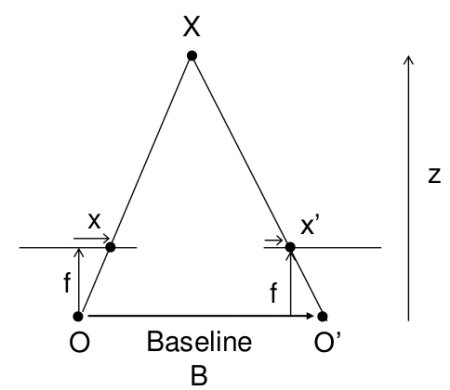
\includegraphics[width=\textwidth]{figures/stereo_depth.jpg}}{Stereo depth}
\caption{Stereo depth}
\label{fig:stereo}
\end{figure}

Stereo analyysillä kuvankäsittelyssä tarkoitetaan kahdesta samasta kohteesta otetusta kuvasta olevien yhtenäisyyksillä syvyyden analysointia.
Vaikka näitä tekniikoita voi varioida mihin tahansa kuviin jotka ovat samasta kohteesta,
tässä yhteydessä käytämme kuvia,
jotka ovat otettu samasta perspektiivistä siten että kuvat ovat horisontaalisesti vierekkäin.
Jos tiedetään kameroiden sijainti toisistaan tai jonkin pisteen etäisyys kamerasta voidaan myös kuvasta arvioida absoluuttinen etäisyys kameraan. 

Kun stereoparia analysoidaan ja tunnistetaan korreloiva piste molemmista kuvista,
voidaan laskea kuvien välinen dispariteetti \ref{fig:stereo}
Tämä tarkoittaa käytännöstä muutosta pisteen sijainnissa kuvien välillä.
Periaatteessa vastaavat pisteet voivat sijaita missä tahansa kuvassa.
Kuitenkin tässä tapauksessa jossa kuvat ovat tietyssä suhteessa toisiinsa,
voidaan olettaa stereoparin löytyvän x akselilta tai ainakin melko läheltä sitä.
Jos näin ei olisi jouduttaisiin kuvan jokaista pistettä vertaamaan jokaiseen pisteeseen toisessa kuvassa.
Tämä tapa tulee nopeasti hyvin kalliiksi.
Jos verrattava alue on myös hyvin pieni todennäköisyys tunnistaa useita samankaltaisia alueita kasvaa.
Jos alue on suuri tai vertailu suoritetaan liian tarkasti,
kasvaa todennäköisyys että vaihtunut kuvakulma on niin erilainen että sitä ei tunnisteta.
Tästä johtuen tämän ongelman ratkaisuun on kehitetty monia erilaisia tapoja.

TODO: Tähän voisi hakea lähteitä. Ihan vaan joku geneerinen stereo analyysi artikkeli.


\subsection{SGM Semi global matching}

Jotta stereo analyysi on mahdollista,
tulee kuvasta tunnistaa samat kohteet.
Yksi tapa tehdä tämä on Hircmuller:in SGM tekniikan avulla\cite{hirschmuller2005babel}.
Tämä tekniikka ottaa huomioon pikselin ja sen ympäröivien pikselien arvot etsiessään toisesta kuvasta vastaavaa arvoa. Tämä hakuoidaan tehdä kaavalla.

\begin{equation}\label{yht:SGM}
    E(d) = \sum_{p} D(p, d_p) + \sum_{q \in \mathcal{N}} R(p, d_p, q, d_q)
\end{equation}

Kaavassa \(D(p, d_p)\) summa funktio käy läpi kaikki kuvan pikselit ja vertaa niitä vertailupikseliin.
Tämä antaa perus arvon yksittäisen pikselin samankaltaisuudelle.

Tämän jälkeen pikselin ympäröiviä pikseleitä verrataan toisiinsa \(R(p, d_p, q, d_q)\).
koska saman asian ympäröivät pikselit tulisi olla melko samankaltaisia molemmissa kuvissa, 
Vaikka se onkin kuvattu hieman eri asennosta, voidaan tämän avulla arvioida onko kyseessä sama piste.

Tämän algoritmin implimentoi pythonin opencv kirjaston SGBM \cite{opencvsgbm},
jota varioitu alkuperäiseen implimentaatioon verrattuna, käymään läpi pikseli joukkoja, eikä yksittäisiä pikseleitä.
Tämä nopeuttaa prosessointia huomattavasti.
Se myöskin suorittaa joitain suodatuksia parempien tulosten saavuttamiseksi.

\section{Neuroverkot}



Tämän työn lopputulos on neuroverkko.
neuroverkko on yleisesti kuva-analyysiin sekä muuhun koneoppimiseen käytettävä tekniikka.
Sen toiminta perustuu neuroneihin joita järjestetään verkkomaiseen rakenteeseen useisiin eri kerroksiin.

Neuroverkko on laskennallinen malli, joka on saanut inss


\begin{equation}\label{yht:neuroni}
    a = \sigma\left(\sum_i w_i x_i + b\right)
\end{equation}

Tämä on neuronin matemaattinen kaava,
se tuottaa ulostulonaan arvon \(a\) saamiensa syötteiden perusteella.
\(x_i\) on neuronin saama syöte.
\(w_i\) on neuronille annettu painoarvo.
\(b\) on neuronin bias arvo. \(\sigma\) on funktio joka muuttaa neuronin saavan armon välille 0,1.

Kun näitä neuroneita asetetaan eri kerroksiin siten että verkon sisääntulo on esimerkiksi valokuvan kokoinen,
ja ulostulo on liukuluku,
voidaan verkolle syöttää kuvia autoista ja asioista jotka eivät ole autoja.
Kun nämä kuvat on oikein luokiteltu, voidaan niillä kouluttaa verkko tunnistamaan autoja.
Koulutuksen aikana verkko muuttaa arvojaan \(w_i\) ja \(b\).
Nämä arvot se saa yrittämällä erilaisia arvoja neuroneille.
Kun verkkoa tämän jälkeen testataan, voidaan saaduista lopputuloksista valita paras.
Tämän jälkeen tätä lopputulosta voidaan lähteä parantelemaan,
testaamalla toimiiko suuremmat vai pienemmät arvot paremmin.
Kun näitä kahta arvoa eri neuroneilla muutetaan,
saadaan joka kierroksella hieman paremmin toimiva verkko.

Neuroverkko on siis vain kasa yksinkertaisia matemaattisia funktioita,
joiden toimintaa muokkaamalla pyritään saamaan haluttu lopputulos.
Jotta lopputulos on koskaan haluttu pitää tätä koulutusprosessia kuitenkin valvoa.
Tämä tapahtuu tappiofunktion (loss function) sekä takaisinvirtausalgoritmin (backpopagation algoKun näitä neuroneita asetetaan eri kerroksiin siten että verkon sisääntulo on esimerkiksi valokuvan kokoinen, ja ulostulo on yhen neuronin ulostulo, voidaan verkolle syöttää kuvia esimerkiksi kissoista ja koirista. Kun näille kuville annetaan arvot 0 ja 1 kuvan aiheen mukaan, voidaan verkko kouluttaa tunnistamaan kissoja ja koiria. Koulutuksen aikana verkko muuttaa arvojaan \(w_i\) ja \(b\). Nämä arvot se saa yrittämällä erilaisia arvoja neuroneille. Kun verkkoa tämän jälkeen testataan on voidaan saaduista lopputuloksista valita paras. Tämän jälkeen tätä lopputulosta voidaan lähteä parantelemaan, testaamalla toimiiko suuremmat vai pienemmät arvot paremmin. Kun näitä kahta arvoa eri neuroneilla muutetaan saadaan paremmin toimiva neuroverkko.

Neuroverkko on siis vain kasa yksinkertaisia matemaattisia funktioita, joiden toimintaa vain tuurilla arvoidaan jotta saadaan haluttu lopputulos. Tätä tuuria pyritään parantamaan ohjaamalla verkon koulutusta. Tämä tapahtuu tappiofunktion (loss function) sekä takaisinvirtausalgoritmin (backpopagation algorithm) avulla. Loss functionin tehtävä on kertoa kuinka paljon saatu tulos eroaa halutusta. Esimerkki tapauksessamme tämä käytännössä katsoisi onko kissa kuvan arvo mikä sen pitäisi olla. Tämän työn lopputulos on verkko joka yrittää luoda kuvasta 3d pistekartan. Siinä tapauksessa siis neliösumma tai jokin muu tapa virheen tunnistamiseen olisi parempi. Kun virhe on tunnistettu verkkoa muokataan takaisinvirtaus algoritmin perusteella. Tähän ei ole yhtä parasta ratkaisua, vaan eri verkkojen ja käyttökohteiden tapauksessa eri algoritmit voivat tuoda huomattavasti parempia tuloksia.
rithm) avulla.
Tappiofunktion tehtävä on kertoa kuinka paljon saatu tulos eroaa halutusta.
Esimerkkitapauksessamme tämä käytännössä testaa, verkon lopputuloksen ja palauttaa kuinka monta arvausta verkko sai oikein.
Virheen tunnistus ei kuitenkaan ole aina yhtä yksinkertaista. 
Jos lopputulos on esimerkiksi kuva, hankaloituu kouluttaminen huomattavasti.
Mitä yksinkertaisempi lopputulos sitä helpompi verkko on kouluttaa.
Kun virhe on tunnistettu, verkkoa muokataan takaisin virtaus algoritmin perusteella.
Tähän ei ole yhtä parasta ratkaisua, vaan eri verkkojen ja käyttökohteiden tapauksessa eri algoritmit voivat tuoda huomattavasti parempia tuloksia.

\section{Semantic segmentation}

Semantic segmentation eli kuvan segmentointi on yleinen käyttökohde neuroverkoille.
Sen avulla on helppo tehdä käytettäviä ja helposti hyödynnettäviä malleja.
Ja se on hyvä esimerkki ongelmasta jolle on helppo tehdä koulutusdataa, mutta hankala luoda ohjelmallista toteutusta saman lopputuloksen saamiseksi.
Esimerkkejä käytöstä on esimerkiksi automatisoidussa liikenteessä,
liikenteen esteiden tunnistamisessa \ref{fig:labels}.
\begin{figure}[h]
\centering
\pdftooltip{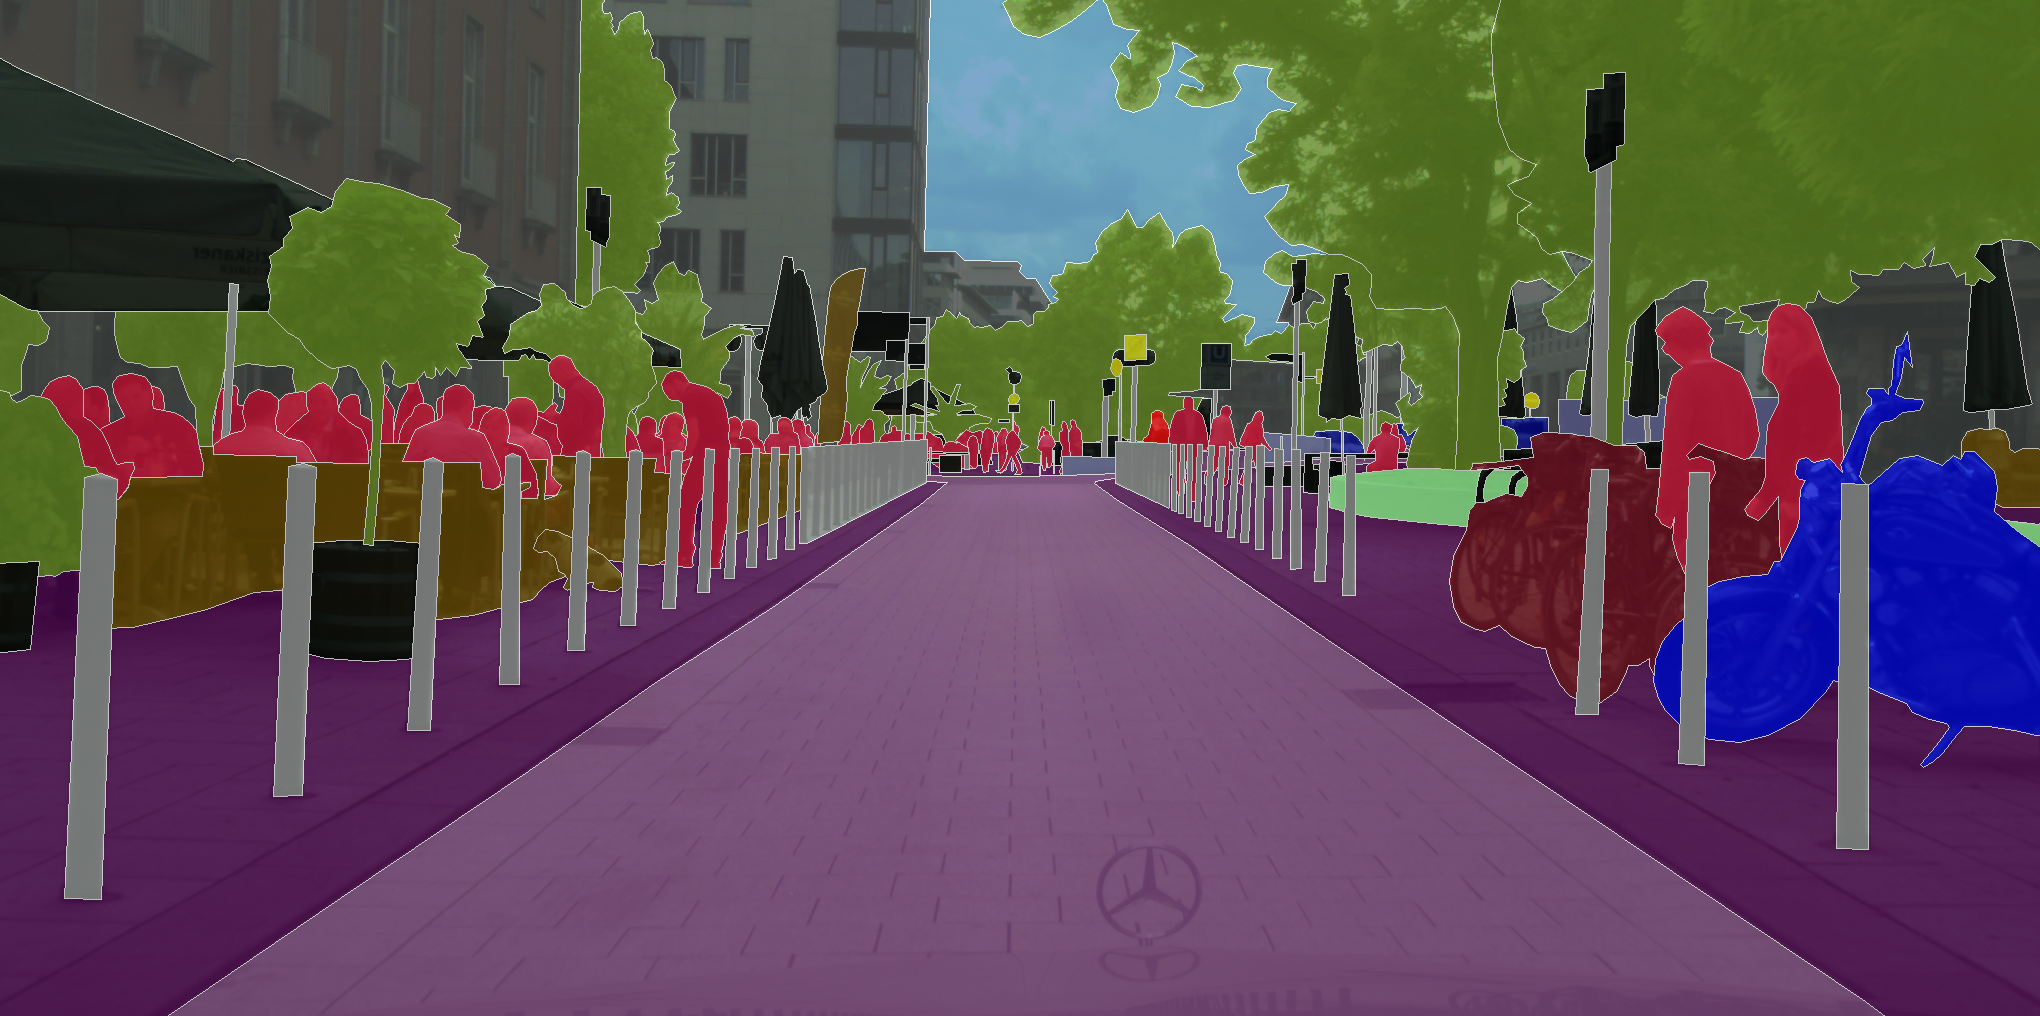
\includegraphics[width=\textwidth]{figures/stuttgart03.png}}{Cityscapes esimerkki kuva stuttgart03}
\caption[Tämä on lyhyt kuvateksti.]{Cityscapes datestin esimerkki segmentointi dataa, jossa kaupunki näkymän erilaiset tunnistattavat kohteet on merkitty eri väreillä.}
\label{fig:labels}
\end{figure}

Tätä teknologiaa voidaan käyttää useiden eri tunnistus ongelmien ratkaisuun.
Koulutusdatasta riippuen kuvasta voidaan tunnistaa mitä tahansa. Samaa teknologiaa käytetään teollisissa applikaatioissa laadun valvonnassa, sekä lääketieteessä erilaisten skannausten analysoinnissa.
Mallin voi kouluttaa tunnistamaan useita tai vain yhtä asiaa riippuen käyttökohteesta.
Toisin kuin perinteinen object detection malli, joka tunnista yleensä vain mitä kuvassa on. Segmnetaatio malli antaa joka pikselille arvon jonka perusteella lopputuloksesta voidaan nähdä, mitä eri kohdissa kuvaa on.
Jotta samanlainen lopputulos saataisiin object detection mallilla pitäisi kuvaa käydä läpi pienemmissä lohkoissa jotta rajat löytyisivät.

Segmentointi mallin kouluttaminen ja datasetin käsittely on kuitenkin hieman haastavampaa kuin object detection mallin. Jotta mallin voi kouluttaa tunnistamaan asiat pikselitasolla, on myös opetusdatan oltava pikselitasolla annotoitua. 
Myöskin datan koulutuksessa käytettävä tappiofunktion määrittely hieman hankaloituu.
Mallin koulutuksessa pitää käyttää jotain muuta tapaa tunnistaa sen onnistuminen, kuin vain ”onko kyseessä auto”.

Yksi koulutuksessa käytettävä tappion laskutapa, jota myös tässä työssä käytetään, on CrossEntropyLoss. Se on yleisesti käytössä semantic segmentation mallien koulutuksessa. 

TODO: Selitä tässä cross entrropy loss https://pytorch.org/docs/stable/generated/torch.nn.CrossEntropyLoss.html

\section{Syvyyskartta}

Tämän työn haluttu lopputulos on syvyyskartta.
Syvyyskartta on yksinkertainen kuvan kaltainen esitystapa, jossa eri syvyyksillä on eri numeerinen arvo.
Se voidaan näyttää esimerkiksi siten että kauempana kamerasta oleva kohde on tummemmalla värillä \ref{fig:depth}.
Tärkeä ero 3d malliin sekä syvyyskartan välillä on datan perspektiivi.
Syvyyskartassa ei ole tietoa kohteiden takana olevasta tilasta, joten sitä voi tarkastella vain sen kuvaus perspektiivistä.


\begin{figure}[h]
\centering
\pdftooltip{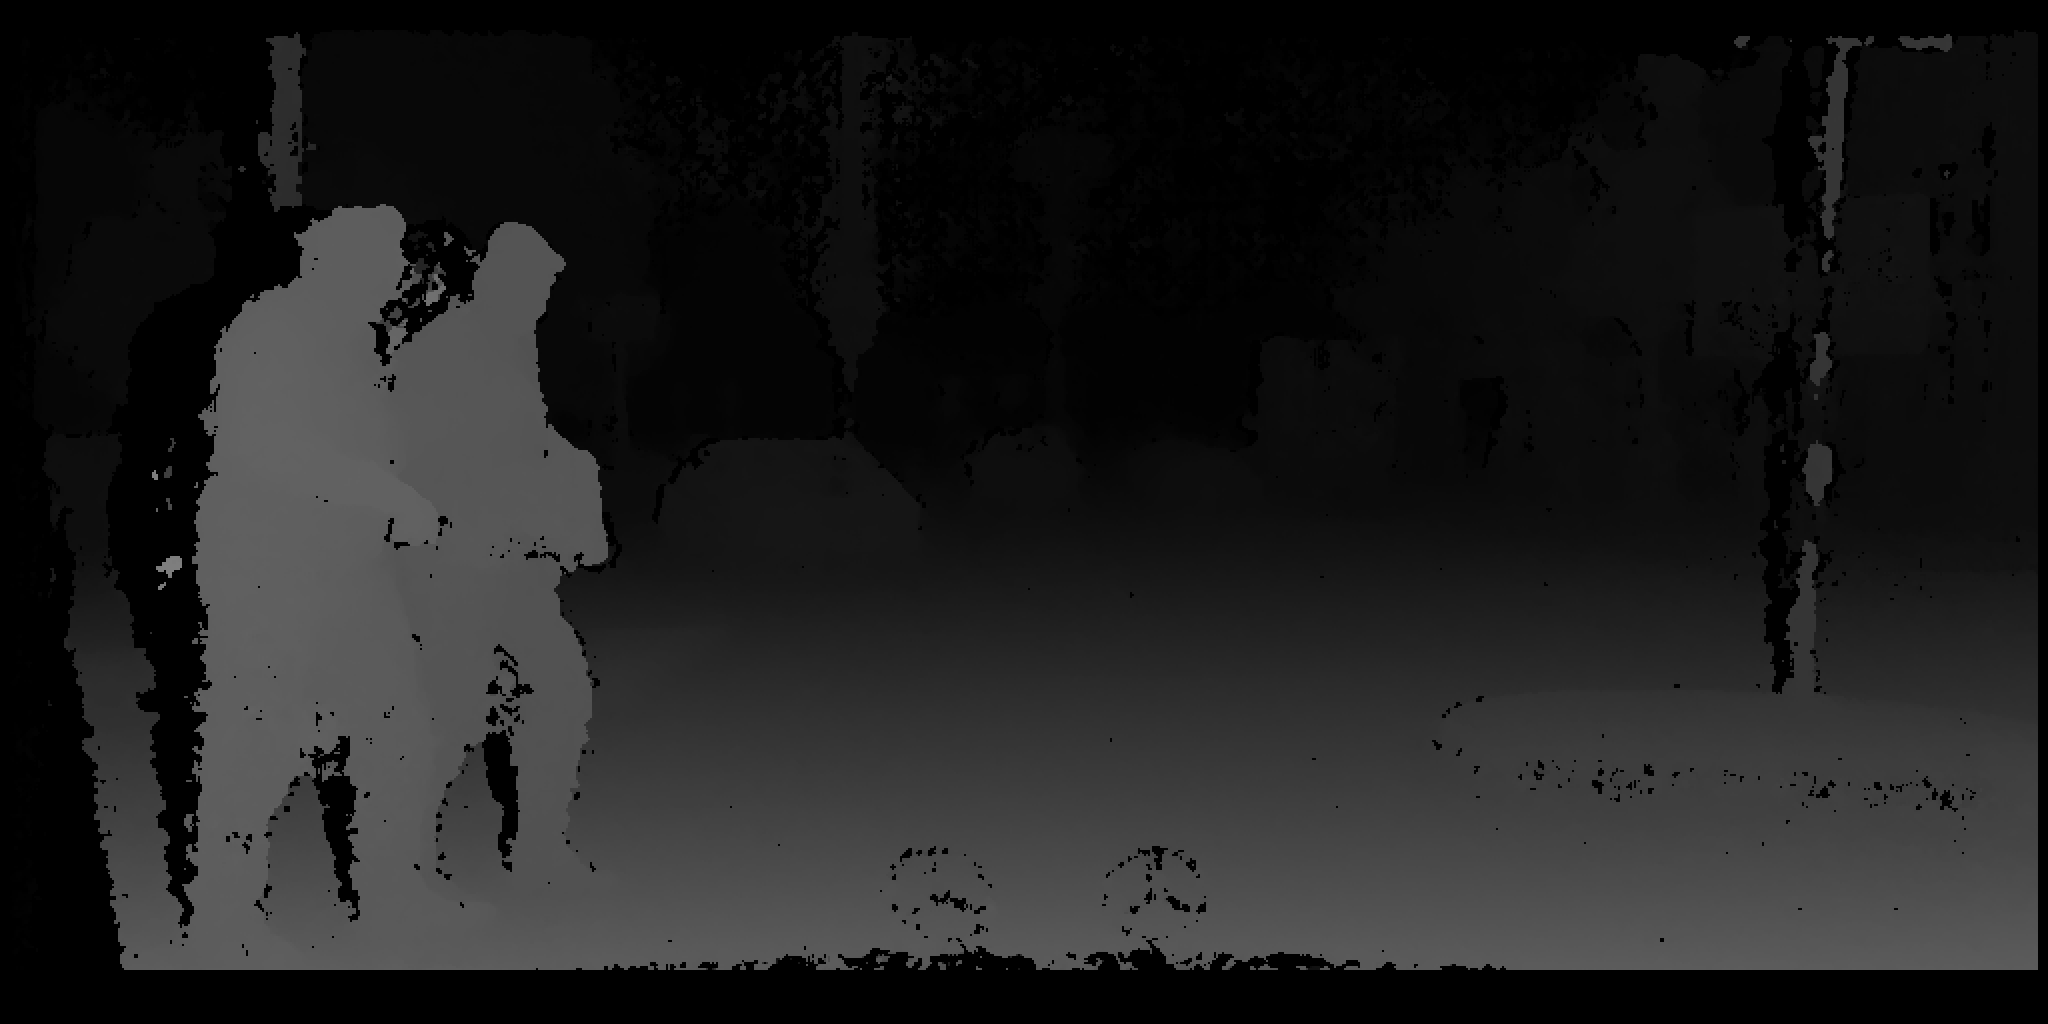
\includegraphics[width=\textwidth]{figures/leverkusen_000024_000019_disparity.png}}{Cityscapes esimerkki kuva leverkusen_000024_000019_disparity}
\caption[Tämä on lyhyt kuvateksti.]{Citysscapes datasetin syvyysdata esimerkki.}
\label{fig:depth}
\end{figure}
